\section{Shade}
        \begin{figure}[!htb]
            \begin{center}
              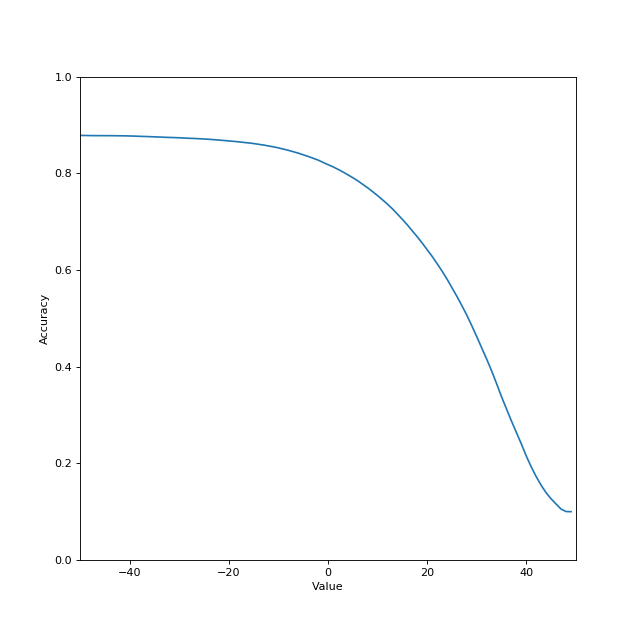
\includegraphics[scale=0.6]{chapters/results/CNN/Shade/acc.png}
              \caption{Overall accuracy for metamorphic relation rotation.}
              \label{fig:Shade 1}
            \end{center}
        \end{figure}
    
    \clearpage
        \begin{figure}[!htb]
        \centering
          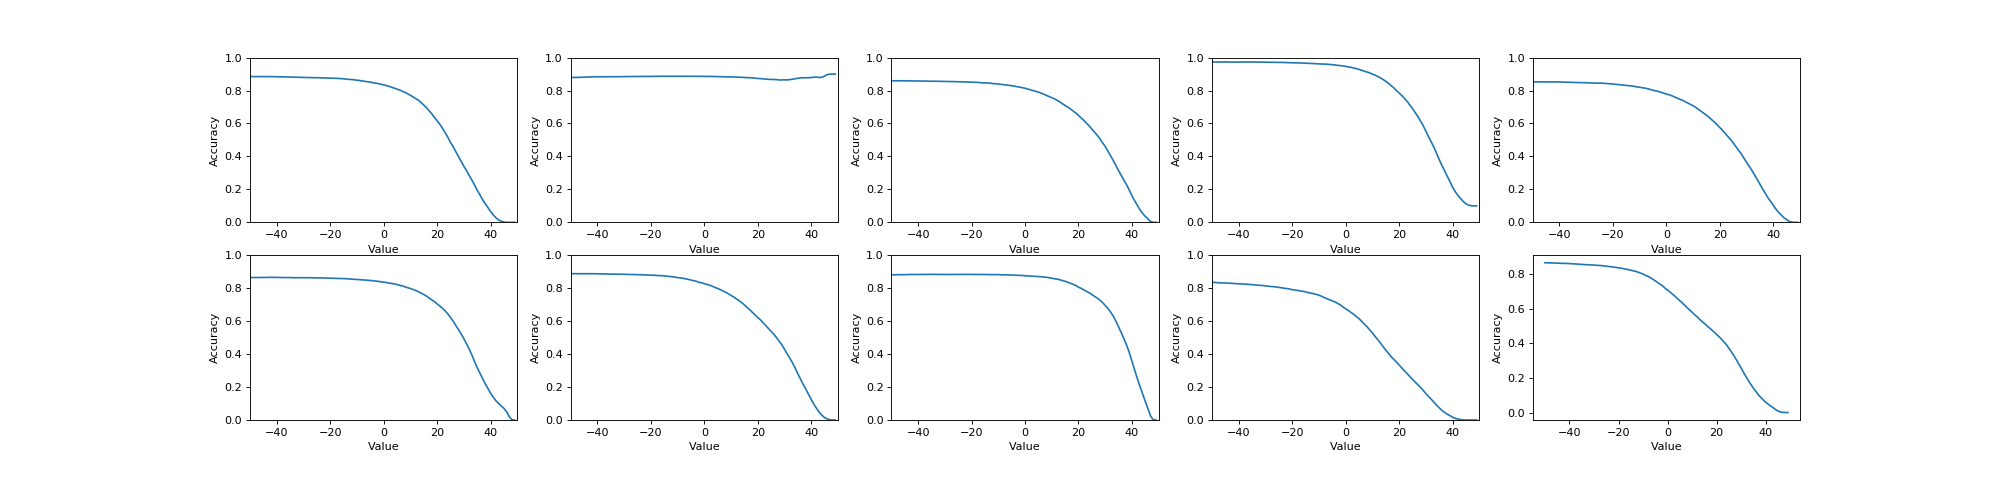
\includegraphics[scale=0.4]{chapters/results/CNN/Shade/accAll.png}
          \caption{Accuracy of each digit for Shade.}
          \label{fig: Shading}
        \end{figure}
        
    \clearpage
    \begin{figure}[htb!]
        \centering
        \begin{subfigure}[b]{\textwidth}
            \centering
            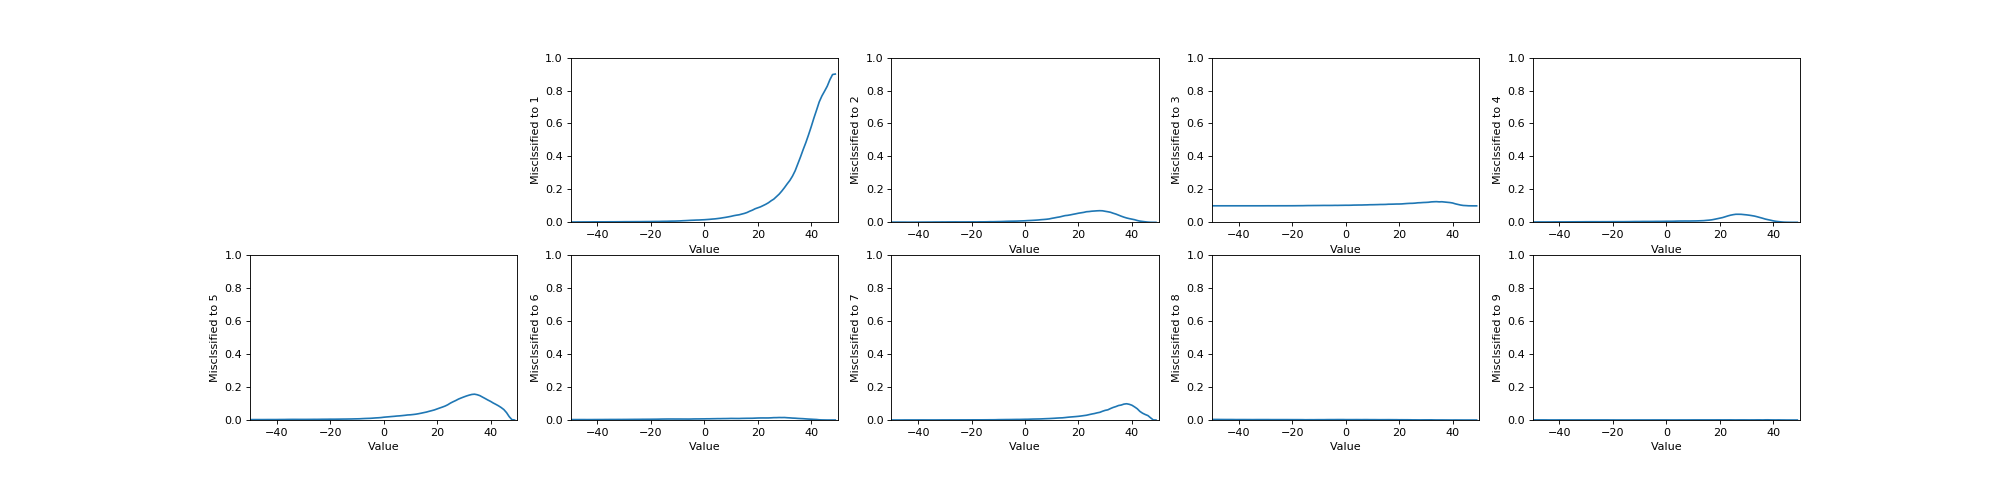
\includegraphics[width=\textwidth]{chapters/results/CNN/Shade/acc1.png}
            \caption{Caption for subfigure 1}
            \label{fig:Shade-misclass0}
        \end{subfigure}
        \begin{subfigure}[b]{\textwidth}
            \centering
            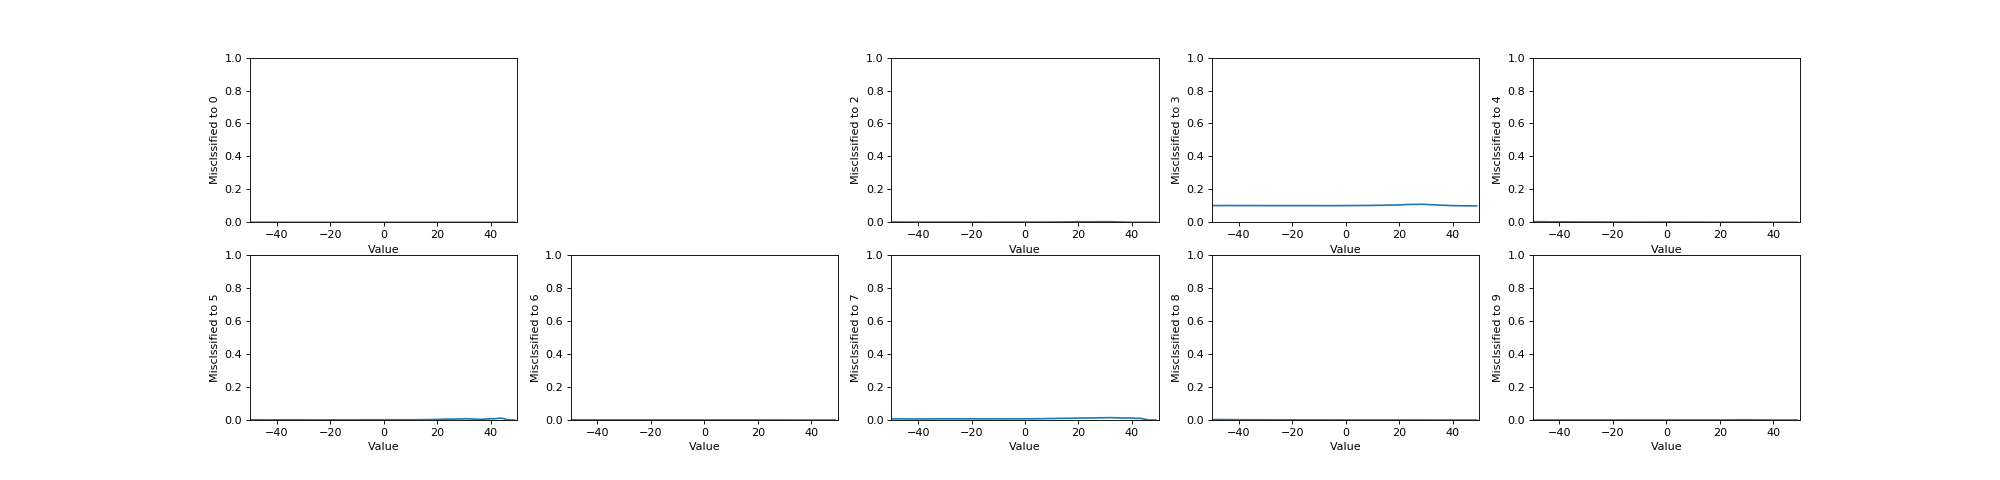
\includegraphics[width=\textwidth]{chapters/results/CNN/Shade/acc2.png}
            \caption{Caption for subfigure 1}
            \label{fig:Shade-misclass0}
        \end{subfigure}
        \begin{subfigure}[b]{\textwidth}
            \centering
            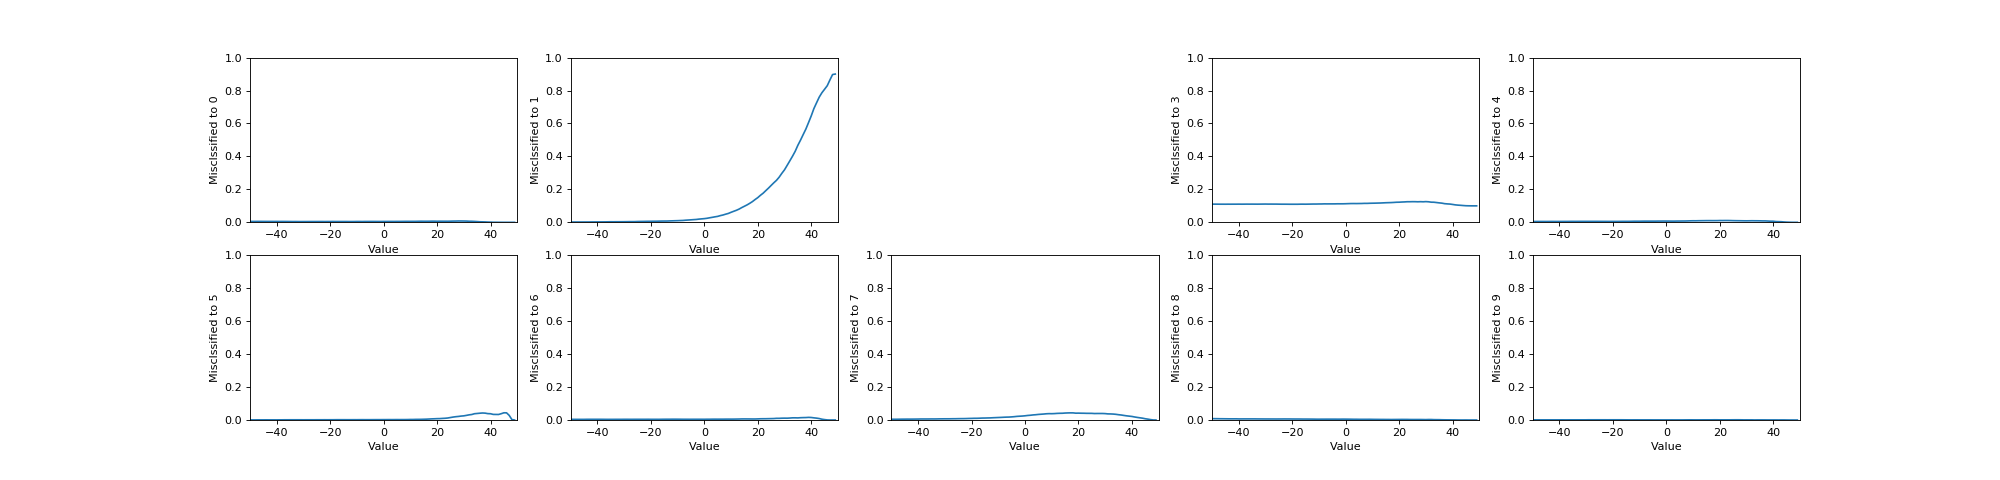
\includegraphics[width=\textwidth]{chapters/results/CNN/Shade/acc3.png}
            \caption{Caption for subfigure 1}
            \label{fig:Shade-misclass0}
        \end{subfigure}
        \begin{subfigure}[b]{\textwidth}
            \centering
            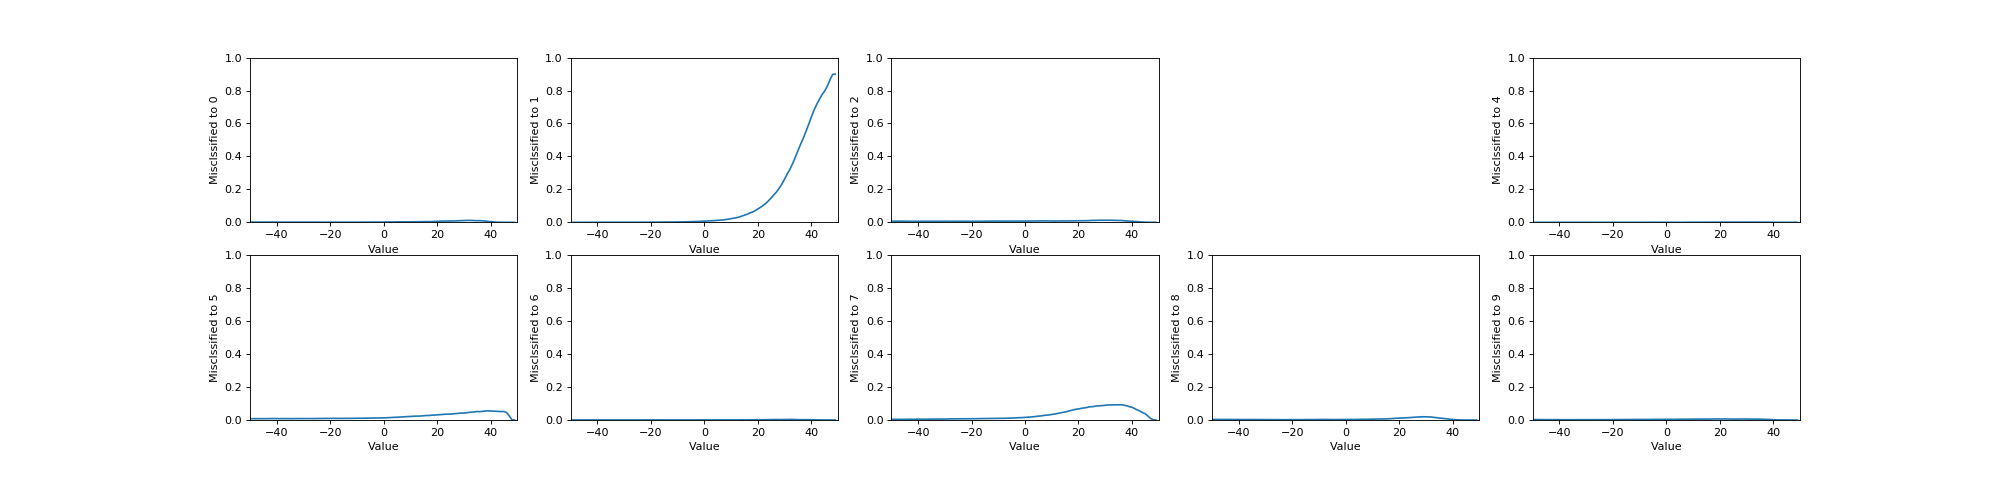
\includegraphics[width=\textwidth]{chapters/results/CNN/Shade/acc4.png}
            \caption{Caption for subfigure 1}
            \label{fig:Shade-misclass0}
        \end{subfigure}
        \begin{subfigure}[b]{ \textwidth}
            \centering
            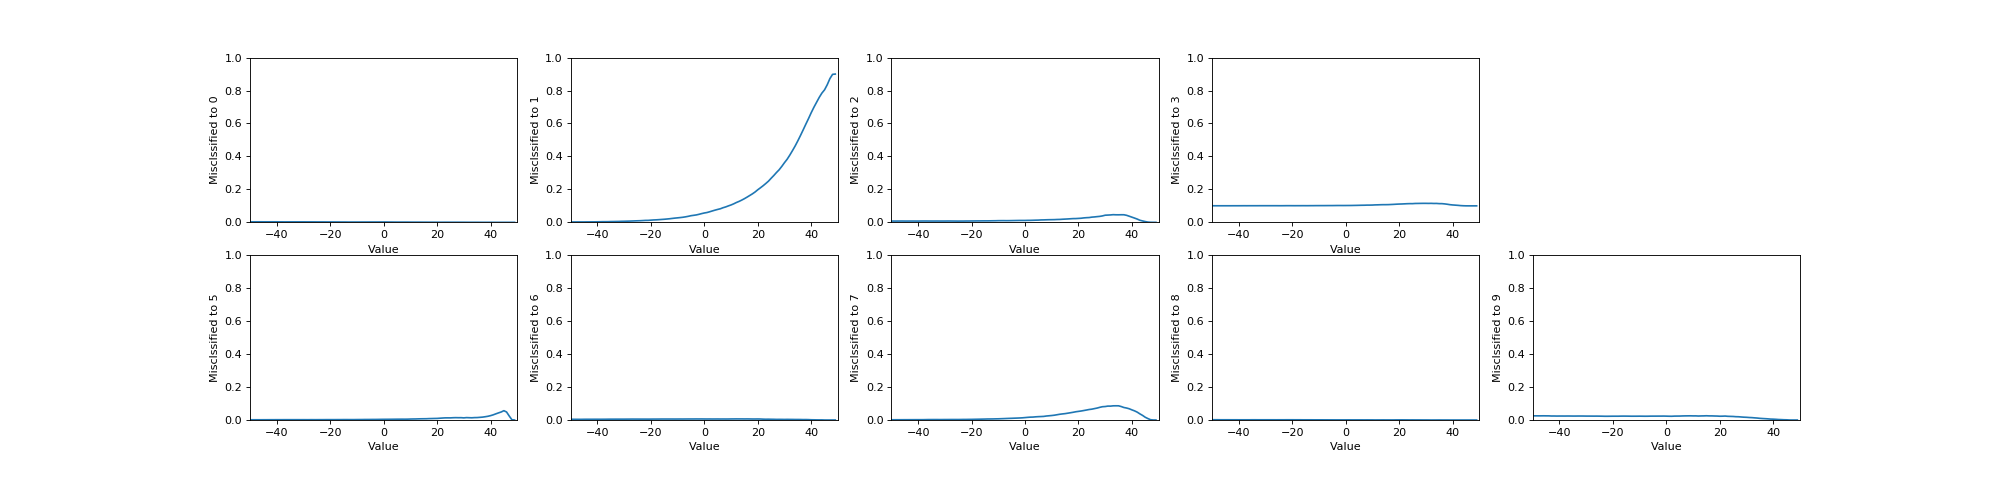
\includegraphics[width=\textwidth]{chapters/results/CNN/Shade/acc5.png}
            \caption{Caption for subfigure 2}
            \label{fig:Shade-misclass1}
        \end{subfigure}
        \caption{Caption for all subfigures.}
        \label{fig:Shade-misclassifications}
    \end{figure}
    
    \clearpage
    \begin{figure}[htb!]
        \centering
        \begin{subfigure}[b]{\textwidth}
            \centering
            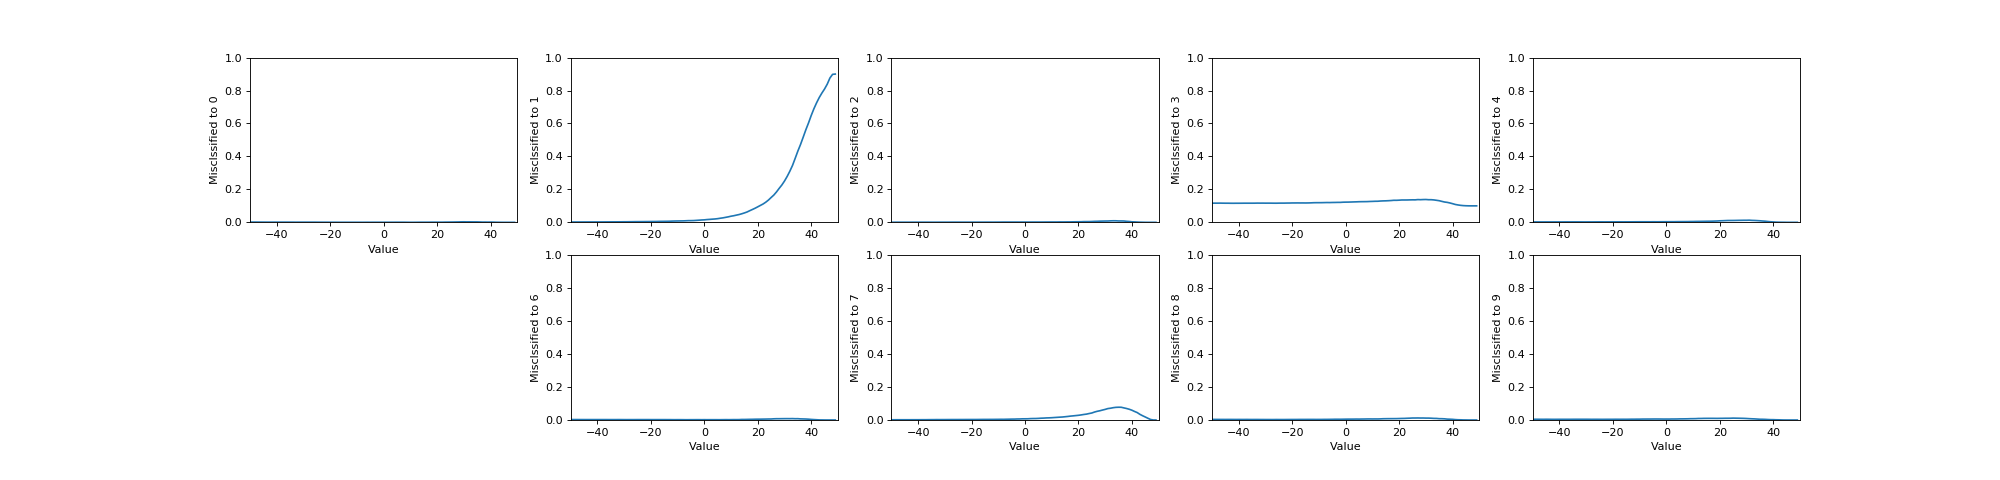
\includegraphics[width=\textwidth]{chapters/results/CNN/Shade/acc6.png}
            \caption{Caption for subfigure 1}
            \label{fig:Shade-misclass0}
        \end{subfigure}
        \begin{subfigure}[b]{\textwidth}
            \centering
            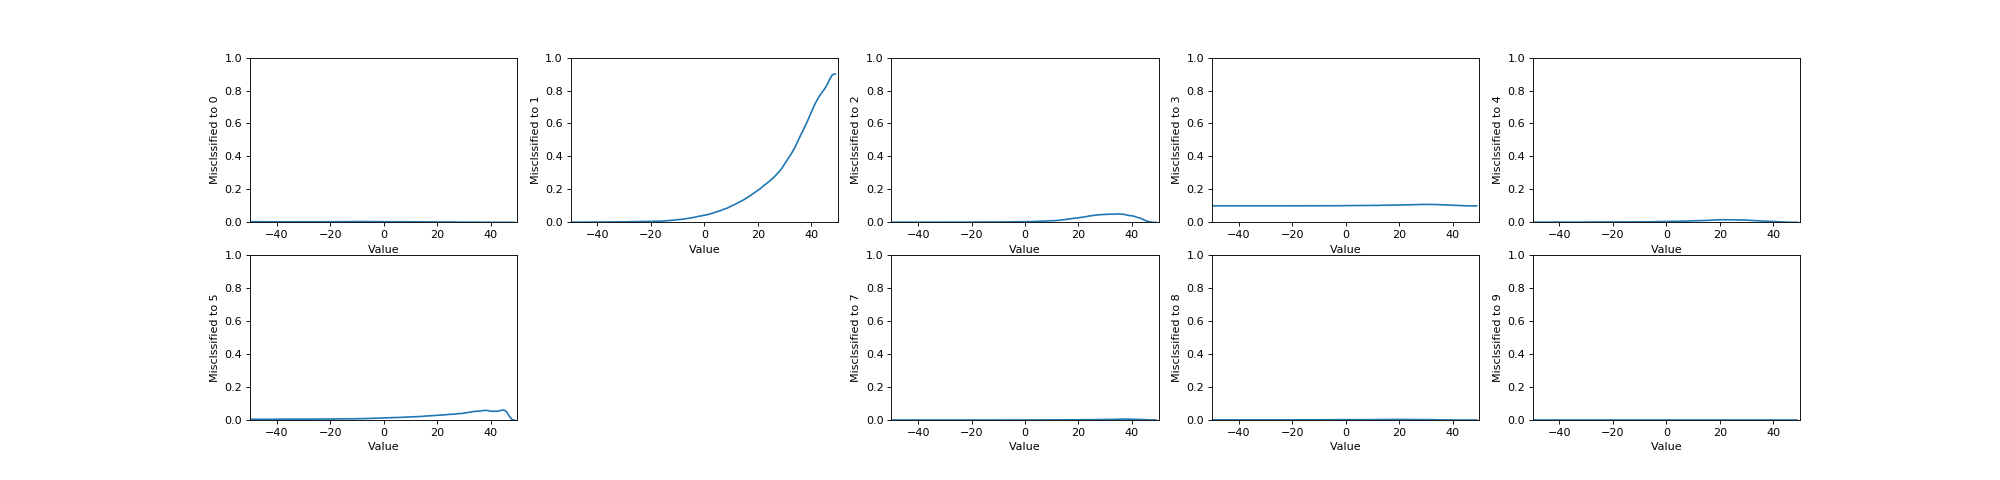
\includegraphics[width=\textwidth]{chapters/results/CNN/Shade/acc7.png}
            \caption{Caption for subfigure 1}
            \label{fig:Shade-misclass0}
        \end{subfigure}
        \begin{subfigure}[b]{\textwidth}
            \centering
            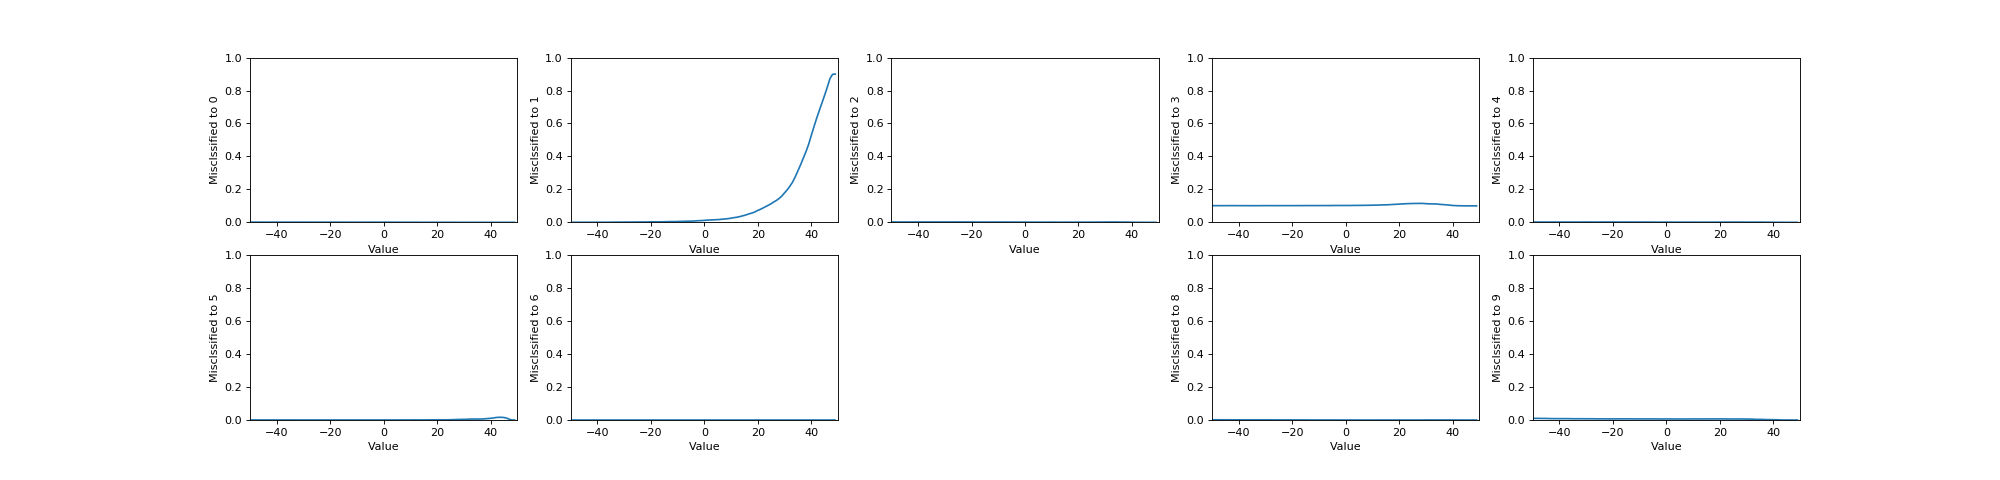
\includegraphics[width=\textwidth]{chapters/results/CNN/Shade/acc8.png}
            \caption{Caption for subfigure 1}
            \label{fig:Shade-misclass0}
        \end{subfigure}
        \begin{subfigure}[b]{\textwidth}
            \centering
            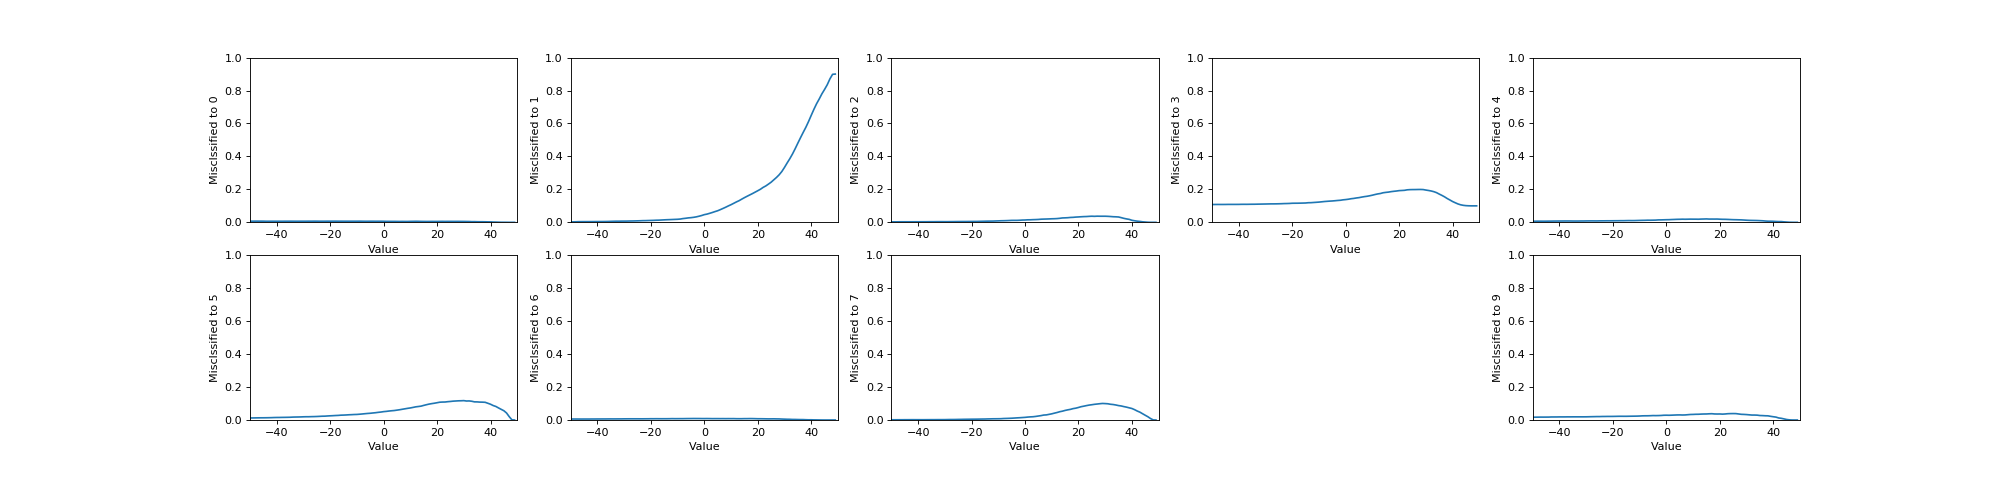
\includegraphics[width=\textwidth]{chapters/results/CNN/Shade/acc9.png}
            \caption{Caption for subfigure 1}
            \label{fig:Shade-misclass0}
        \end{subfigure}
        \begin{subfigure}[b]{ \textwidth}
            \centering
            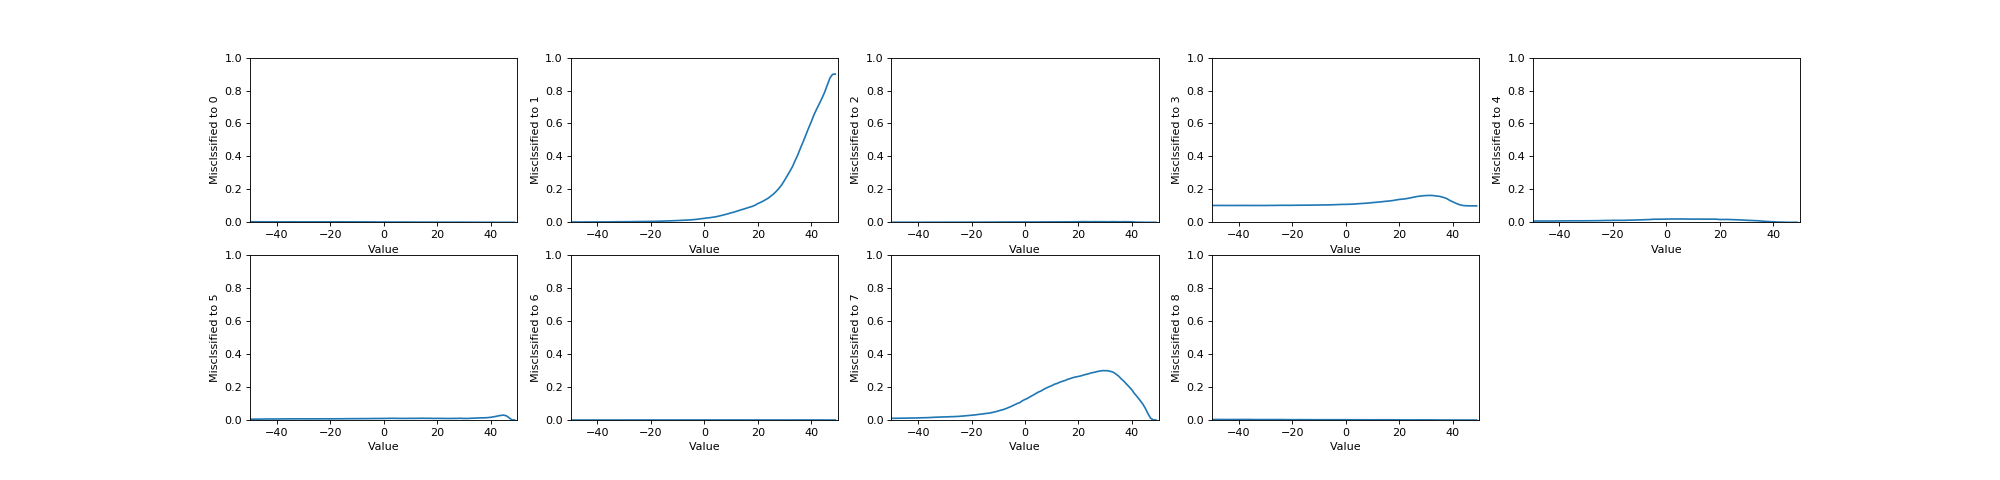
\includegraphics[width=\textwidth]{chapters/results/CNN/Shade/acc10.png}
            \caption{Caption for subfigure 2}
            \label{fig:Shade-misclass1}
        \end{subfigure}
        \caption{Caption for all subfigures.}
        \label{fig:Shade-misclassifications}
    \end{figure}
        
\clearpage
